\newpage
\section{RESULT AND DISCUSSION}
\subsection{Current Result}
% Table
During Training We calculated PSNR and SSIM for Set5 datasets at every epoch for both SRResNet and SRGAN.
\begin{figure}[h]
    \centering
    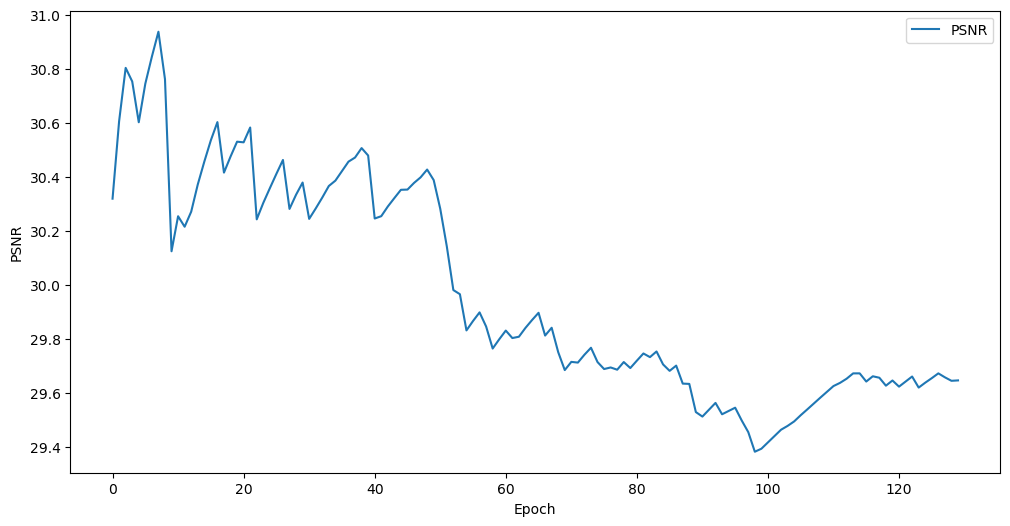
\includegraphics[width=5.5in]{./figures/srresnet_psnr.png}
    % \caption{SRResNet PSNR Plot}
    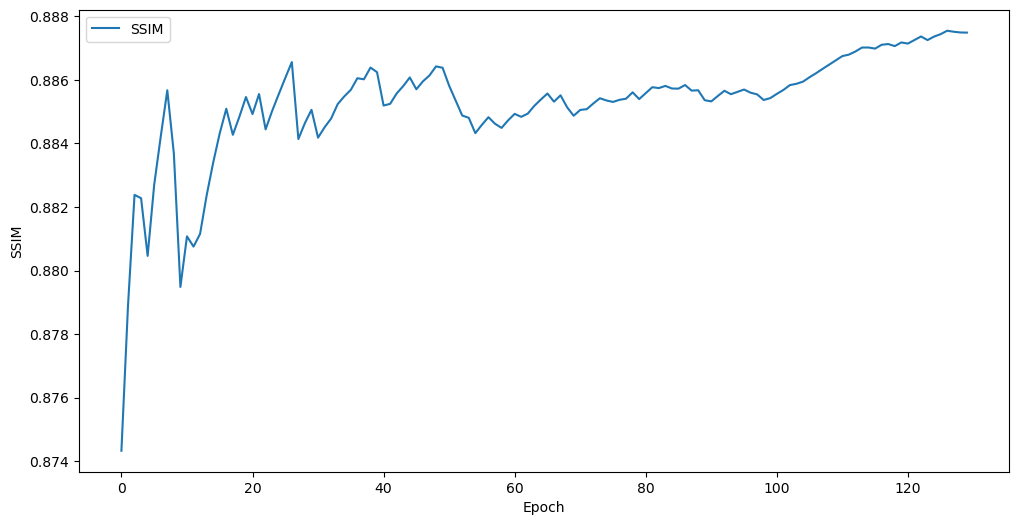
\includegraphics[width=5.5in]{./figures/srresnnet_ssim.png}
    \caption{SRResNet PSNR and SSIM Plot for Set5}
\end{figure}  
\begin{figure}[h]
    \centering
    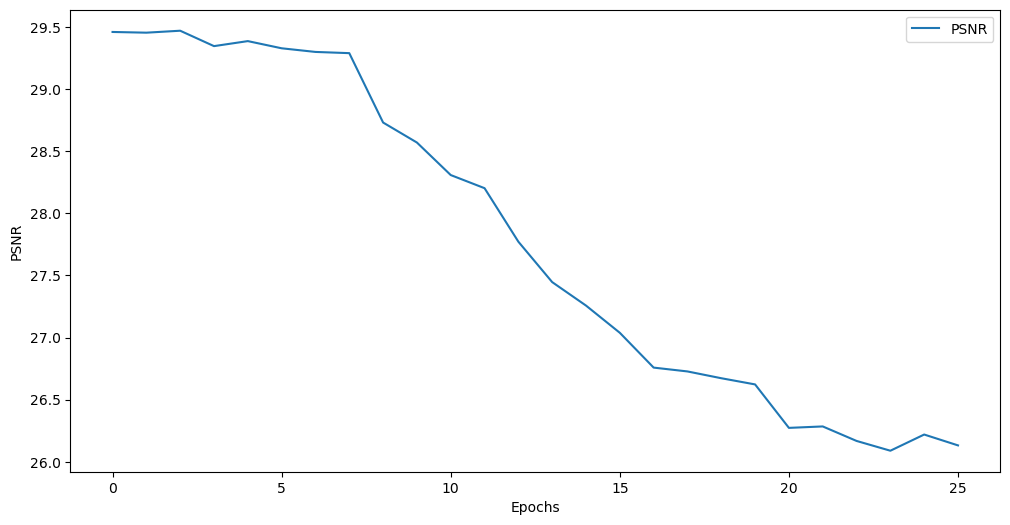
\includegraphics[width=5.5in]{./figures/srgan_psnr.png}
    % \caption{SRResNet PSNR Plot}
    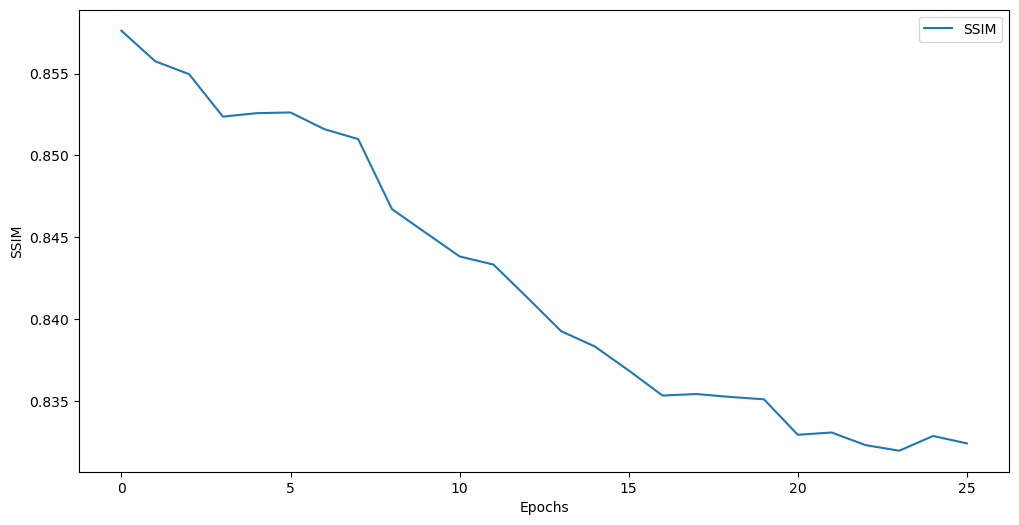
\includegraphics[width=5.5in]{./figures/srgan_ssim.png}
    \caption{SRGAN PSNR and SSIM Plot for Set5}
\end{figure}  
\begin{figure}[h]
    \centering
    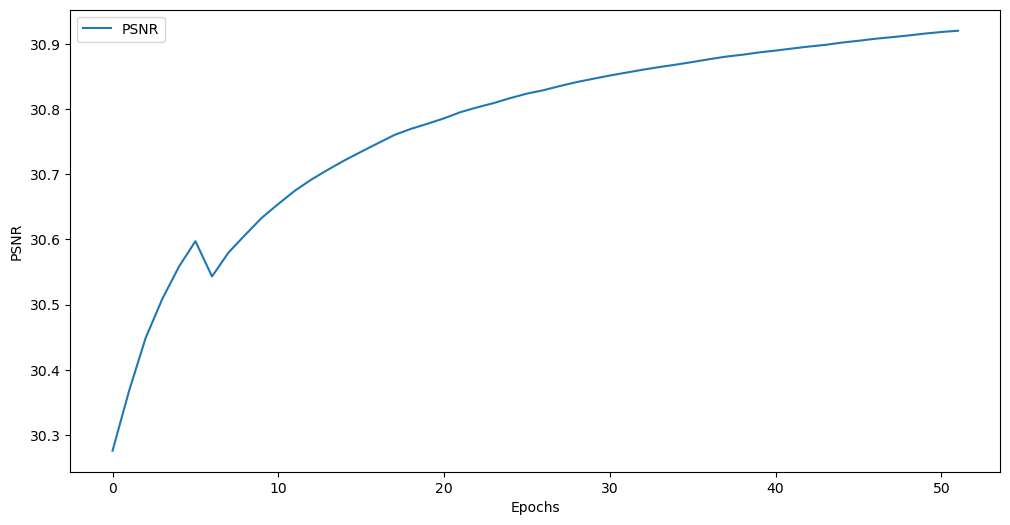
\includegraphics[width=5.5in]{./figures/SRCNN_PSNR.png}
    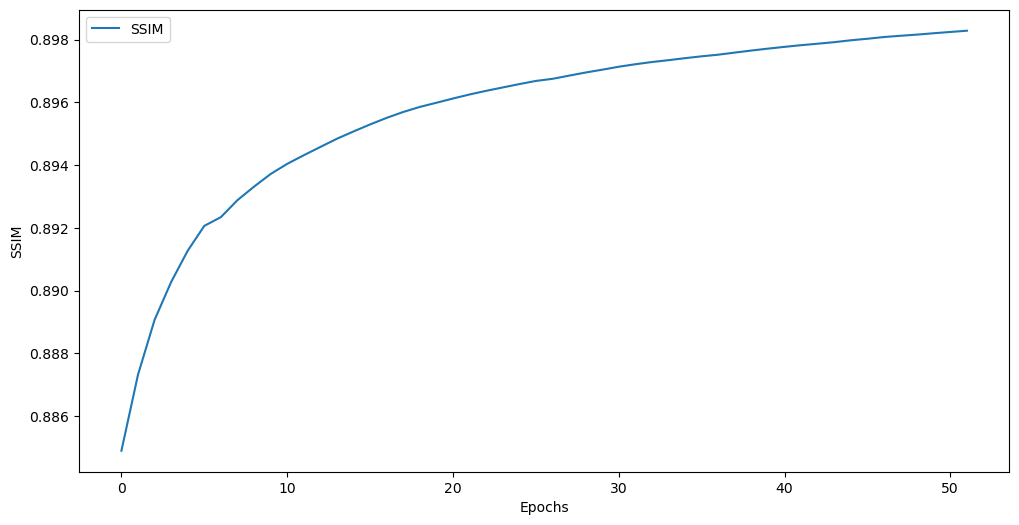
\includegraphics[width=5.5in]{./figures/SRCNN_SSIM.png}
    \caption{SRCNN PSNR and SSIM Plot for Set5}
\end{figure} 
    These metrics don't actually match with human perception but even if PSNR and SSIM is decreasing they are becoming more stable and we see model get better after each epoch.
%  \clearpage
%  \newpage
    We have also calculated PSNR and SSIM for all the test datasets Set5, Set14 and BSDS100 after the training was completed.
\begin{table}[h]
    \centering
    \begin{tabular}{|c|c|c|c|c|c|c|}
    \hline
    &PSNR & SISM & PSNR & SISM & PSNR & SISM \\
    \hline
    SRCNN(3x)&31.02 & 0.9 & 27.668 & 0.812 & 26.939 & 0.781 \\
    \hline
    SRCNN(4x)&28.751 & 0.844 & 25.72 & 0.734 & 25.44 & 0.696 \\
    \hline
    ResNet&29.83 & 0.887 & 28.275 & 0.795 & 27.203 & 0.751 \\
    \hline
    SRGAN &23.946 & 0.821 &25.112 & 0.715 & 24.631 & 0.662 \\
    \hline
    & \multicolumn{2}{|c|}{Set5}& \multicolumn{2}{|c|}{Set14} & \multicolumn{2}{|c|}{BSD100} \\
    \hline
    \end{tabular}
    \caption{Evaluation Metrics in Test Datasets}
\end{table}
\clearpage
\newpage
    These are the few results from comparing Bicubic, SRResNet and SRGAN super resolved images with the original HR images.
    \begin{figure}[t]
        \centering
        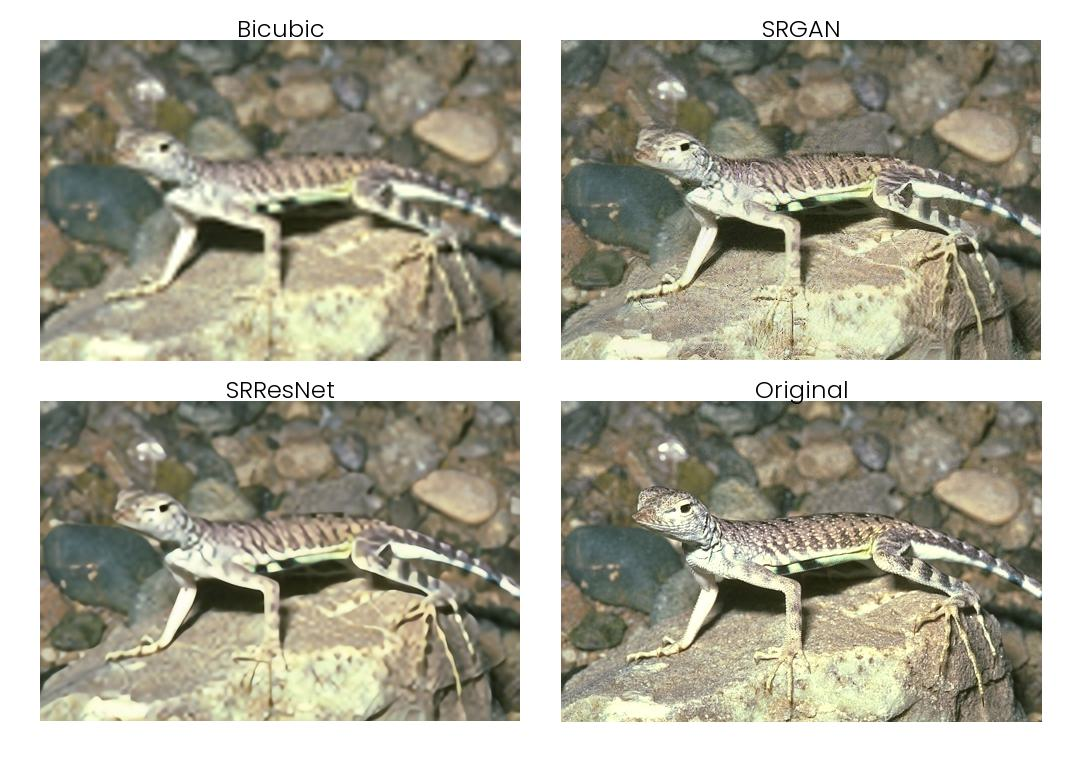
\includegraphics[width=5.5in]{./figures/examples/lizard.jpg}
        \caption{Image of super resolved lizard with SRResNet, SRGAN and HR image}
    \end{figure}
    \begin{figure}
        \centering
        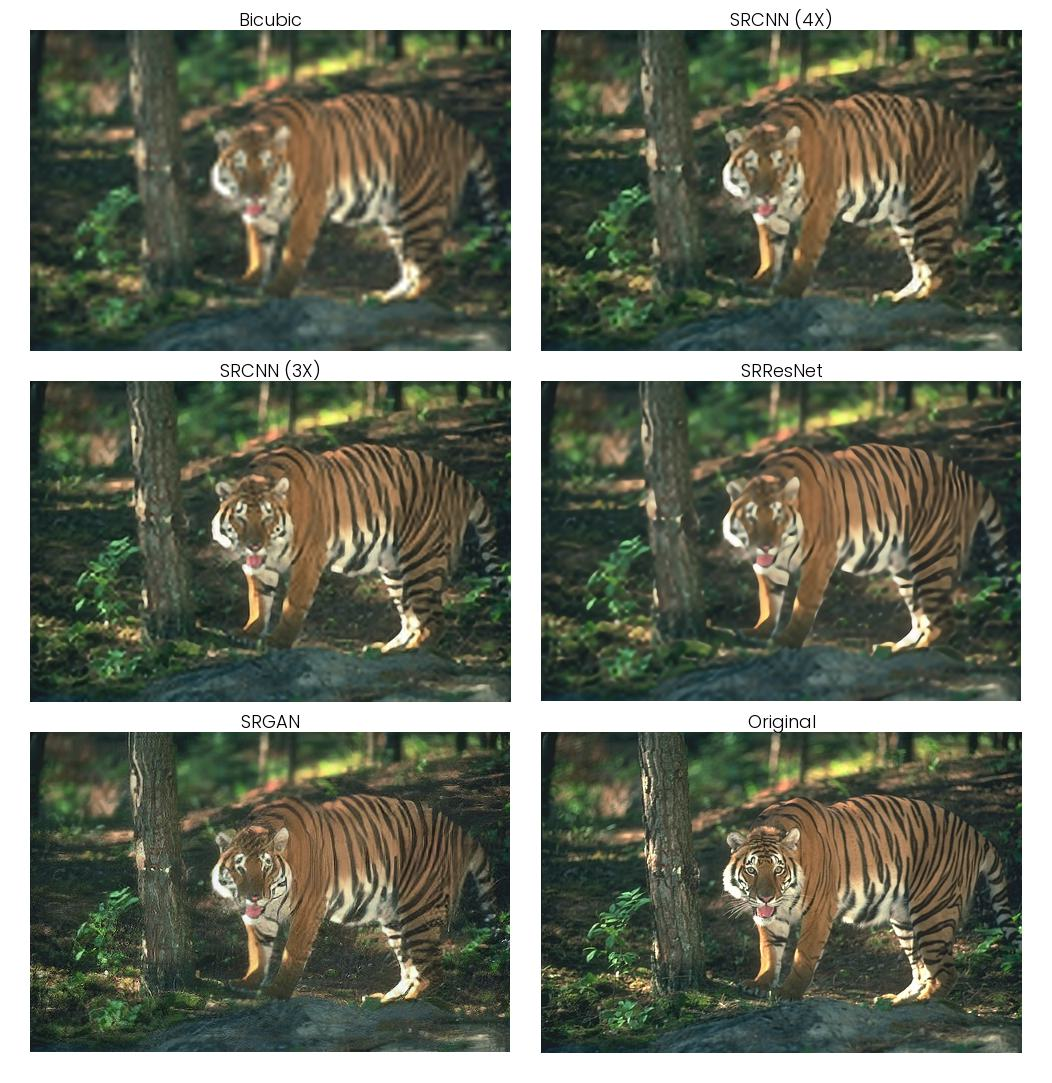
\includegraphics[width=5.5in]{./figures/examples/tiger.jpg}
        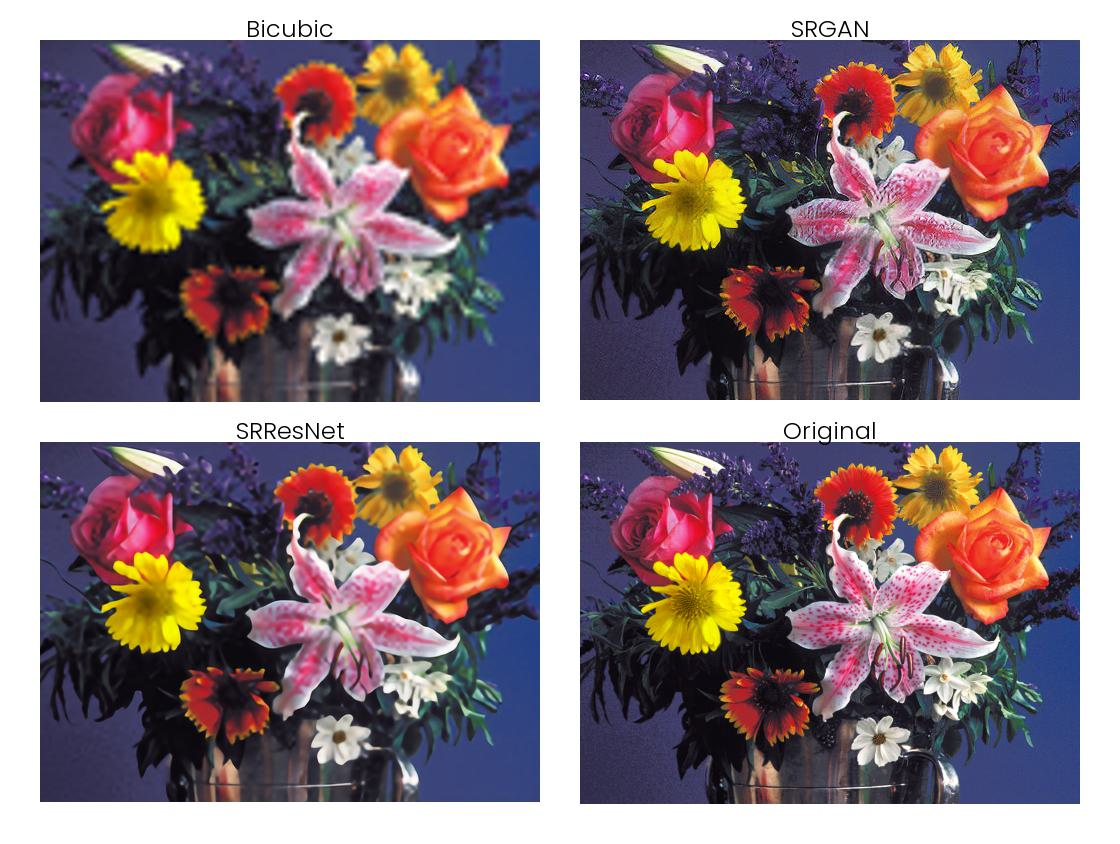
\includegraphics[width=5.5in]{./figures/examples/flowers.jpg}
        \caption{Images of super resolved flowers and tiger with SRResNet, SRGAN and HR image}
    \end{figure}      
  
\clearpage
\newpage
\subsection{Work Completed:}
As we are planning on comparison of different methods. We have selected few methods like SRCNN, SRGAN, and ESRGAN. SRGAN involves residual network SRResNet which will be also used as baseline for SRGAN. We have trained and tested SRGAN on various sets of data involving CelebA, DIV2k, Flickr2k, OST and COCO(2014). CoCo has a large and diverse set of data and it perfromed well thats why we are finalizing this dataset for training further methods. 
\subsection{Work Remaining}
\begin{enumerate}
    \item We have not trained models for SRCNN and ESRGAN yet.
    \item We don't have a polished website to showcase our results.
\end{enumerate}  
\subsection{Limitations}
Few limitations related to SRGAN that we have trained are:
\begin{enumerate}
    \item The implementation and training of SRGAN demand substantial computational resources, posing challenges in terms of the time and hardware needed.
    \item  The effectiveness of SRGAN relies heavily on the availability of a sizable and diverse training dataset, presenting challenges in obtaining and curating such data.
    \item There is a lot of subjectivity in evaluating the images as quantitative metrics can't identify human perception.
    \item  The study lacks comparison with real-world benchmarks or scenarios.
    \item Due to constraints, we couldn't explore tinkering hyperparameters.
    \item The study lacks a direct comparison with the latest state-of-the-art super-resolution techniques.
\end{enumerate}
% \subsection{Problem Faced}
% \subsection{Budget Analysis}
\subsection{Work Schedule:}
\newcolumntype{P}[1]{>{\raggedright\vrule height4ex width 0pt}p{#1}<{\vrule depth 2.5ex width 0pt}}
    \begin{tabular}{|P{6cm}*{10}{|c}|}
    \hline
    \centering \raisebox{-2ex}[0pt][0pt]{Action plan} & \multicolumn{7}{c|}{2023} & \multicolumn{3}{c|}{2024} \\
    \cline{2-11}
    \multicolumn{1}{|c|}{\vphantom{$\Big|$}} &
    \scriptsize Jun & \scriptsize Jul & \scriptsize Aug & \scriptsize Sep &
    \scriptsize Oct & \scriptsize Nov & \scriptsize Dec & \scriptsize Jan &
    \scriptsize Feb & \scriptsize Mar \\
    \hline
    Research &
    {\cellcolor{gray}} &{\cellcolor{gray}}&{\cellcolor{gray}}&{\cellcolor{gray}}&{\cellcolor{gray}}&&&&& \\
    \hline
    Data Acquisition &
    && {\cellcolor{gray}} &{\cellcolor{gray}} &{\cellcolor{gray}} &&&&& \\
    \hline
    Model Development and Evaluation &
    &&&&{\cellcolor{gray}} &{\cellcolor{gray}}&{\cellcolor{gray}}&&& \\
    \hline
    Model Deployment &
    &&&&&&{\cellcolor{gray}}&{\cellcolor{gray}}&{\cellcolor{gray}} & \\
    \hline
    Prepare the report and presentation &
    &&&&&&{\cellcolor{gray}}&{\cellcolor{gray}}&{\cellcolor{gray}}&{\cellcolor{gray}} \\
    \hline
    \end{tabular}